\documentclass[a4paper, 12pt]{article}
\usepackage[a4paper,top=1.0cm, bottom=0.5cm, left=0.25cm, right=0.75cm]{geometry}
\usepackage[utf8]{inputenc}
\usepackage{mathtext}
\usepackage{amsmath}
\usepackage{amsfonts}
\usepackage[english, russian]{babel}
\usepackage{indentfirst}
\usepackage{longtable}
\usepackage{graphicx}
\graphicspath{{pictures/}}
\DeclareGraphicsExtensions{.pdf,.png,.jpg}


\title{Лабораторная работа 2.5.1 Измерение коэффициента поверхностного натяжения жидкости.
       \vspace*{19 cm}}
\author{Трунов Владимир}
\date{8 марта 2022 г.
      \newpage}

\newpage

\begin{document}
    \newpage
	\maketitle
	\section*{Цель работы}
		1) измерение температурной зависимости  коэффициента поверхностного натяжения дистиллированной воды с использованием известного коэффициента поверхностного натяжения спирта;  \\
        2) определение полной поверхностной энергии  и теплоты, необходимой для изотермического образования единицы  поверхности жидкости  при различной температуре.
	\section*{Оборудование}
		Прибор Ребиндера с термостатом и микроманометром, спирт и вода, стакан.
	\section*{Теория к работе}
		Наличие поверхностного слоя приводит к различию давлений по разные стороны от искривленной границы раздела двух сред.  Для сферического пузырька с воздухом  внутри жидкости избыточное давление даётся формулой Лапласа: 
		$$\Delta P = P_{внутри} - P_{снаружи} = \frac{2 \sigma}{R}$$
		$\sigma$ - коэффициент поверхностного натяжения, $R$ - радиус кривизны поверхности раздела двух фаз. Измеряется давление $\Delta P$, необходимое для выталкивания в жидкость пузырька воздуха. 
	\section*{Описание экспериментальной установки}
		На рисунке ниже изображена экспериментальная установка. Исследуемая жидкость(дистиллиро- ванная вода) наливается в сосуд(колбу) В. Тестовая жидкость(этиловый спирт) наливается в сосуд Е. При измерениях колбы герметично закрываются пробками. Через одну из двух пробок проходит полая металлическая игла С. Этой пробкой закрывается сосуд, в котором проводятся измерения. Верхний конец иглы открыт в атмосферу, а нижний погружён в жидкость. Другой сосуд герметично закрывается второй пробкой. При создании достаточного разряжения воздуха в колбе с иглой пузырьки воздуха начинают пробулькивать через жидкость. Поверхностное натяжение можно определить по величине разряжения $\Delta P$, необходимого для прохождения пузырьков(при известном радиусе иглы).
		\\
		\\
		Разряжение в системе создается с помощью аспиратора А. Кран К2 разделяет две полости аспиратора. При закрытом кране К2 открывают кран К1, разряжение воздуха в колбе создаётся когда вода вытекает из крана К1 по каплям. В колбах В и С, соединённых трубками с нижней полостью аспиратора, создается такое же пониженное давление. Разность давлений в полостях с разряженным воздухом и атмосферой измеряется спиртовым микроманометром. Для стабилизации температуры исследуемой жидкости через рубашку D колбы В непрерывно прогоняется вода из термостата. 
		\begin{figure}[h]
			\center{\includegraphics{exp}}
		\end{figure}
		\\
		\\
		Обычно кончик иглы лишь касается поверхности жидкости, чтобы исключить влияние гидростатического давления столба жидкости. Однако при измерении температурной зависимости коэффициента поверхностного натяжения возникает ряд сложностей. Во-первых, большая теплопроводность металлической трубки приводит к тому, что температура на конце трубки заметно ниже, чем в глубине жидкости. Во-вторых, тепловое расширение поднимает уровень жидкости при увеличении температуры.
		\\
		\\
		Обе погрешности можно устранить, погрузив кончик трубки глубже в жидкость. Полное давление, измеренное при этом микроманометром, $P = \Delta P + \rho gh$. $\rho gh$ не зависит от температуры жидкости. Величину $\rho gh$ следует измерить двумя способами. Во-первых, замерить величину $Р1= \Delta P'$, когда кончик трубки только касается поверхности жидкости. Затем при этой же температуре опустить иглу глубже в жидкость и замерить $Р2 = \rho gh + \Delta P"$ ($\Delta P'$, $\Delta P"$ – давление Лапласа). Из-за несжимаемости жидкости можно положить $\Delta P'= \Delta P"$ и тогда $\rho gh = Р2 - Р1$. Во-вторых, при измерениях Р1 и Р2 замерить линейкой глубину погружения иглы h.
		
	\section*{Ход работы}
        Для начала опустим кончик иглы в спирт и установим скорость капель примерно 1 капля в 5 секунд.
        Далее проведем измерение максимального давления при пробулькивании пузырька. Далее промоем иглу и проведем аналогичные измерение для поверхности воды.
        После этого погрузим кончик иглы на максимально возможную глубину и установим зависимость коэффициента поверхностного натяжения от темпетаруты.
        \\  
		Измерим $d = 2R = 1,20 \pm 0,05$мм - диаметр иглы с помощью микроскопа.
		Разность давлений измеряется не напрямую, а через положение жидкости в манометре, поэтому $\Delta P = k h$, где h - высота в миллиметрах жидкости в манометре, а $k = 1,96 \frac{Па}{мм}$ - коэффициент пересчёта. 
        Погружать иголку будем на $H$ = 6,5 см. Измеренные данные занесём в таблицу:
		\begin{longtable}[H]{|c|c|c|c||c|c|c|c|}
			\hline
			Жидкость & h, мм & $P$, Па & $\overline{\Delta P}$, Па & Жидкость & h, мм & $P$, Па & $\overline{\Delta P}$, Па \\
			\hline
			& 41 & 80,36 & &  & 130 & 254,80 & \\
			& 40 & 78,40 & &  & 131 & 256,76 & \\
			Спирт(23,4 °C) & 39 & 76,34 & 78,32 & Поверхность воды(23,4 °C) & 130 & 254,80 & 254,80 \\
			& 40 & 78,40 & &  & 129 & 252,84 & \\
			& 40 & 78,40 & &  & 130 & 254,80 & \\
			\hline
			& 165 & 323,40 & &  & 164 & 321,44 & \\
			& 166 & 325,36 & &  & 165 & 323,40 & \\
			Вода(23,4 °C) & 165 & 323,40 & 323,40 & Вода(28,2 °C) & 163 & 319,48 & 321,44\\
			& 164 & 321,44 & &  & 164 & 321,44 & \\
			& 165 & 323,40 & &  & 164 & 321,44 & \\
			\hline
			& 163 & 319,48 & &  & 162 & 317,52 & \\
			& 163 & 319,48 & &  & 162 & 317,52 & \\
			Вода(34,2 °C) & 164 & 321,44 & 319,48 & Вода(39,2 °C) & 162 & 317,52 & 317,52\\
			& 163 & 319,48 & &  & 163 & 319,48 & \\
			& 162 & 317,52 & &  & 161 & 315,56 & \\
			\hline
			& 161 & 315,56 & &  & 159 & 311,64 & \\
			& 160 & 313,60 & &  & 159 & 311,64 & \\
			Вода(44,2 °C) & 159 & 311,64 & 313,60 & Вода(49,2 °C) & 160 & 313,60 & 311,64 \\
			& 160 & 313,60 & &  & 158 & 309,68 & \\
			& 160 & 313,60 & &  & 159 & 311,64 & \\
			\hline
			& 158 & 309,68 & &  & 157 & 307,72 & \\
			& 157 & 307,72 & &  & 157 & 307,72 & \\
			Вода(54,2 °C) & 158 & 309,68 & 308,90 & Вода(59,2 °C) & 157 & 307,72 & 307,33 \\
			& 158 & 309,68 & &  & 157 & 307,72 & \\
			& 157 & 307,72 & &  & 156 & 305,76 & \\
			\hline
		\end{longtable}
		Из таблицы находим $\rho gh = 68,60\: Па$. Также из данного коэффициента поверхностного натяжения для этилового спирта находим, что диаметр трубки равен $d_{сп}=1,12$ мм. Погрешность составила 7$\%$. Из разности высот иглы рассчитаем $\rho gh_2 = 63,7$ Теперь построим таблицу зависимости $\sigma (T)$. 
        Погрешность нахождения $\sigma$ складывается из погрешностей измерения давление и диаметра иглы и равна $\Delta \sigma = 0,33$ мН/м. 
        При положении иглы у поверхности воды $\sigma = 76,2 \pm 0,33 {мН/м}$, что не совпадает с табличным значением $\sigma = 71,97 {мН/м}$ в пределах погрешости.
		\begin{longtable}[H]{|c|c|c|c|c|c|c|c|c|}
			\hline
			T, °C & 23,4 & 28,2 & 34,2 & 39,2 & 44,2 & 49,2 & 54,2 & 59,2\\
			\hline
			$\sigma$, мН/м & 76,20 & 75,84 & 75,26 & 74,67 & 73,50 & 72,91 & 72,09 & 71,62\\
			\hline
		\end{longtable}
	
		Построим график зависимости $\sigma (T)$:
		
		\begin{figure}[h]
			\center{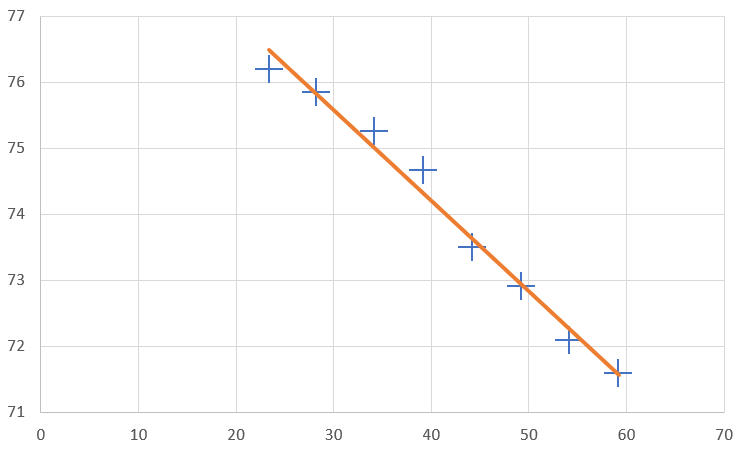
\includegraphics{S(T)}}
		\end{figure}
	
		По этому графику можно найти $\frac{d \sigma}{dT} = -0,13 \pm 0,06\: \frac{мН}{м \cdot K}$. Табличное значение составляет -0,17 $\frac{мН}{м \cdot K}$. Теперь на другом графике построим q(T) и $\frac{U}{F} (T)$: \newpage
		\begin{figure}[h]
			\center{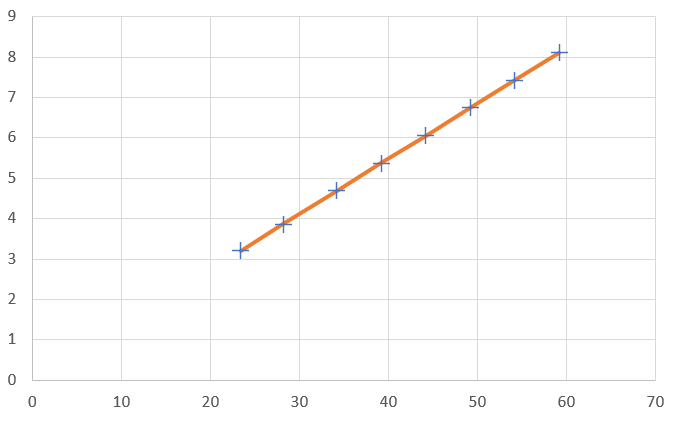
\includegraphics{q(T)}}
		\end{figure}
        \begin{figure}[h]
			\center{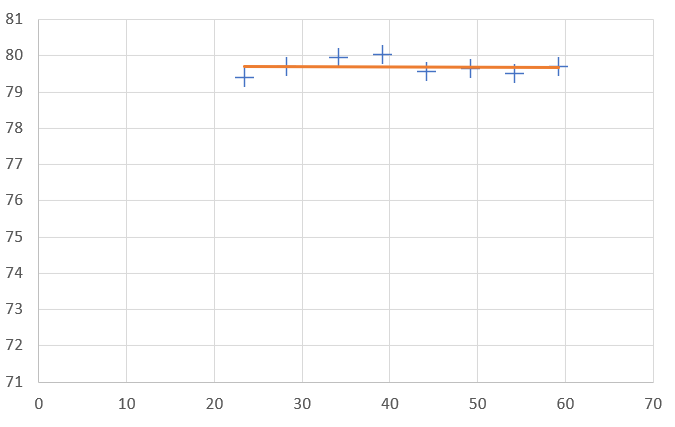
\includegraphics{U(T)}}
		\end{figure}
	\section*{Вывод}
		Нам удалось измерить зависимость коэффициента поверхностного натяжения от температуры. Значение $\frac{d \sigma}{dT}$ и $\sigma$ не сошлись с табличным, однако разница было не очень велика (меньше порядка). Неточности можно объяснить несовершенной чистотой дистиллята и погрешностями измерений (в частности диаметра иглы). Также удалось определить зависимости полной поверхностной энергии и теплоты, необходимой для изотермического образования единицы поверхности жидкости от температуры и построить их графики. 
\end{document}